\documentclass[pdftex]{beamer}
%\input{vc}
% 1.77778 is the ratio of 16 to 9
%\setlength{\paperheight}{3.5in}
%\setlength{\paperwidth}{1.77778\paperheight}
% 1.33333 is the ratio of 4 to 3
\setlength{\paperheight}{4.0in}
\setlength{\paperwidth}{1.33333\paperheight}
% textwidth
\setlength{\textwidth}{0.85\paperwidth}
% import the next thing *after* the papersize
\usepackage{amssymb,amsmath,mathrsfs}
\usecolortheme{default}

% this one is debatable
\renewcommand{\emph}[1]{\textbf{#1}}

%%% color commands
\newcommand{\whiteonblack}{%
  \colorlet{fg}{white}
  \colorlet{bg}{black}
  \setbeamercolor{normal_text}{fg=white,bg=black}
  \setbeamercolor{background canvas}{fg=white,bg=black}
  \setbeamercolor{alerted_text}{fg=yellow}
  \setbeamercolor{example_text}{fg=white}
  \setbeamercolor{structure}{fg=white}
  \setbeamercolor{palette_quaternary}{fg=white}
}
\newcommand{\blackonwhite}{%
  \colorlet{fg}{black}
  \colorlet{bg}{white}
  \setbeamercolor{normal_text}{fg=black,bg=white}
  \setbeamercolor{background canvas}{fg=black,bg=white}
  \setbeamercolor{alerted_text}{fg=blue}
  \setbeamercolor{example_text}{fg=black}
  \setbeamercolor{structure}{fg=black}
  \setbeamercolor{palette_quaternary}{fg=black}
}
\xdefinecolor{pink}{rgb}{1.0,0.9,0.9}

%%% size and shape commands
\newlength{\figurewidth}
\setlength{\figurewidth}{0.9\textwidth}
\newlength{\figureheight}
\setlength{\figureheight}{0.9\textheight}

%%% text commands
\newcommand{\project}[1]{\textsl{#1}}
  \newcommand{\an}{\project{Astrometry.net}}
  \newcommand{\euclid}{\project{Euclid}}
  \newcommand{\flickr}{\project{flickr}}
  \newcommand{\gaia}{\project{Gaia}}
  \newcommand{\galex}{\project{GALEX}}
  \newcommand{\kepler}{\project{Kepler}}
  \newcommand{\GALEX}{\galex}
  \newcommand{\hst}{\project{HST}}
  \newcommand{\hipparcos}{\project{Hipparcos}}
  \newcommand{\lsst}{\project{LSST}}
  \newcommand{\sdss}{\project{SDSS}}
  \newcommand{\sdssiii}{\project{SDSS-III}}
  \newcommand{\sdssiv}{\project{SDSS-IV}}
  \newcommand{\boss}{\project{BOSS}}
  \newcommand{\apogee}{\project{APOGEE}}
  \newcommand{\osss}{\project{OSSS}}
  \newcommand{\ska}{\project{SKA}}
  \newcommand{\vo}{\project{VO}}
  \newcommand{\rttd}{\project{Right Thing To Do}$^{\mbox{\scriptsize\sffamily{TM}}}$}
\newcommand{\foreign}[1]{\textit{#1}}
\newcommand{\latin}[1]{\foreign{#1}}
  \newcommand{\cf}{\latin{cf.}}
  \newcommand{\eg}{\latin{e.g.}}
  \newcommand{\etal}{\latin{et~al.}}
  \newcommand{\etc}{\latin{etc.}}
  \newcommand{\ie}{\latin{i.e.}}
  \newcommand{\vs}{\latin{vs.}}

%%% math-mode commands
\newcommand{\unit}[1]{\mathrm{#1}}
  \newcommand{\rad}{\unit{rad}}
  \newcommand{\s}{\unit{s}}
  \newcommand{\yr}{\unit{yr}}
  \newcommand{\km}{\unit{km}}
  \newcommand{\kmps}{\km\,\s^{-1}}
\newcommand{\mmatrix}[1]{\boldsymbol{#1}}
\newcommand{\tv}[1]{\boldsymbol{#1}}
\newcommand{\dd}{\mathrm{d}}
\newcommand{\given}{\,|\,}
 % hogg standard colors

\newcommand{\credits}{{\footnotesize (Ness, Hogg, \etal)}}
\newcommand{\teff}{T_{\mathrm{eff}}}
\newcommand{\logg}{\log g}
\newcommand{\feh}{[\mathrm{Fe / H}]}

\title{Data-driven models of stars}
\author[David W. Hogg (NYU)]{David W. Hogg \\
  \textsl{\small Center for Cosmology and Particle Physics,
                 New York University} \\
  \textsl{\small Center for Data Science,
                 New York University} \\
  \textsl{\small Max-Planck-Insitut f\"ur Astronomie, Heidelberg}}
\date{2015 April 08}

\newcommand{\conclusions}{%
\begin{frame}
  \frametitle{conclusions}
  \begin{itemize}
  \item A data-driven label transfer system provides \apogee\ stars with labels comparable in quality to the \apogee\ physics-driven pipeline.
    \begin{itemize}
    \item \tc\ (Ness \etal, \textit{ApJ} submitted)
    \item ``labels'' $\equiv (\teff,\logg,\feh)$
    \end{itemize}
  \item \tc\ uses \emph{no physical model of stars}.
  \item The method and the training set are both immature zeroth steps.
  \item There is hope for a consistent system of stellar parameters and chemical abundances across all future surveys.
    \begin{itemize}
    \item \gaia\ \& \project{Gaia-ESO}
    \item \sdssiii\ \project{SEGUE} \& \apogee; \sdssiv\ \project{APOGEE-2}
    \item \project{HERMES} / \project{GALAH}
    \end{itemize}
  \item \texttt{\giturl}
  \end{itemize}
\end{frame}}

\begin{document}

\begin{frame}
  \titlepage
  in collaboration with:\\
  \emph{Melissa~Ness}~(MPIA), {\small Hans-Walter~Rix~(MPIA), \\
  Anna~Ho~(MPIA), Gail~Zasowski~(JHU), and Dan~Foreman-Mackey~(NYU)}
\end{frame}

%\conclusions

\begin{frame}
  \frametitle{Annie Jump Cannon}
  \begin{itemize}
  \item O B A F G K M
    \begin{itemize}
    \item temperature sequence!
    \item alphabetical order (A B F G K M O) is hydrogen-line-strength order
    \end{itemize}
  \item Cannon understood the temperature sequence of stars without the benefit of physical models
    \begin{itemize}
    \item data-driven non-linear dimensionality reduction
    \item ``manifold learning''
    \item (using a huge amount of prior knowledge)
    \end{itemize}
  \item namesake of \tc
  \end{itemize}
\end{frame}

\begin{frame}
  \frametitle{chemodynamics}
  \begin{itemize}
  \item stars populate orbits in the Milky Way
    \begin{itemize}
    \item conserved ``actions''
    \item (or chaotic equivalents)
    \end{itemize}
  \item stars are formed from particular gas clouds
    \begin{itemize}
    \item each cloud has its own history of supernovae
    \item stars have conserved surface abundances
    \item detailed chemical fingerprint
    \item stars that formed together should share a chemical fingerprint
    \end{itemize}
  \item the combined action-chemical space will be far more
    informative than either taken independently
  \end{itemize}
\end{frame}

\begin{frame}
  \frametitle{chemodynamics}
  \begin{itemize}
  \item top priority for many new projects
    \begin{itemize}
    \item \gaia\ \& \project{Gaia-ESO}
    \item \project{HERMES} \& \project{GALAH}
    \item \sdssiii\ \apogee
    \end{itemize}
  \item terrifying inconsistencies in current approaches
    \begin{itemize}
    \item models of stars are \emph{amazingly good}\ldots
    \item \ldots but chemical signatures are \emph{incredibly tiny}
    \end{itemize}
  \end{itemize}
\end{frame}

\begin{frame}
  \frametitle{exoplanets}
  \begin{itemize}
  \item extra-solar planets are always measured relative to their host stars
  \item you only understand a planet \emph{as well as you can understand the star}
  \end{itemize}
\end{frame}

\begin{frame}
  \frametitle{the paradox of precision astrophysics}
  \begin{itemize}
  \item models are incredibly \emph{explanatory}
    \begin{itemize}
    \item $\Lambda$CDM
    \item stellar spectroscopy
    \item helioseismology
    \end{itemize}
  \item and yet...
  \item<2-> models are \emph{wrong} (ruled out) in detail
    \begin{itemize}
    \item $\chi^2 \gg \nu$
    \item ``The $\chi^2$ statistic is a measure of the size of your data!''
    \end{itemize}
  \item<2-> missing physics, approximation, computation, \emph{gastrophysics}
  \end{itemize}
\end{frame}

\begin{frame}
  \frametitle{physics-driven models}
  \begin{itemize}
  \item put in everything you know
    \begin{itemize}
    \item gravity, atomic and molecular transitions, radiation
    \end{itemize}
  \item make approximations to make things computable
    \begin{itemize}
    \item ``sub-grid'' models, mixing length, etc
    \end{itemize}
  \end{itemize}
\end{frame}

\begin{frame}
  \frametitle{machine learning}
  \begin{itemize}
  \item the most extreme of data-driven models
  \item ``the data \emph{is} the model''
    \begin{itemize}
    \item none of your knowledge is relevant
    \end{itemize}
  \item learn (fit) an exceedingly flexible model
    \begin{itemize}
    \item explain or cluster the data
    \item transformation from data to ``labels''
    \end{itemize}
  \item concept of non-parametrics
  \item concept of train, validate, and test
  \item many packages and implementations to choose from
    \begin{itemize}
    \item (and outrageous successes)
    \end{itemize}
  \end{itemize}
\end{frame}

\begin{frame}
  \frametitle{when does machine learning help you?}
  \begin{itemize}
  \item train \& test situation
  \item training data are statistically identical to the test data
    \begin{itemize}
    \item same noise amplitude
    \item same distance or redshift distribution
    \item same luminosity distribution
    \item \emph{never true!}
    \end{itemize}
  \item training data have accurate and precise labels
  \item therefore, we \emph{can't use vanilla machine learning!}
    \begin{itemize}
    \item (astronomers rarely can)
    \end{itemize}
  \end{itemize}
\end{frame}

\begin{frame}
  \frametitle{data-driven models (my personal usage)}
  \begin{itemize}
  \item make use of things you \emph{strongly believe}
    \begin{itemize}
    \item noise model \& instrument resolution
    \item causal structure (shared parameters)
    \end{itemize}
  \item capitalize on huge amounts of data
  \item exceedingly flexible model
  \item concept of train, validate, and test
  \item every situation will be \emph{bespoke}
  \end{itemize}
\end{frame}

\begin{frame}
  \frametitle{label transfer for stars}
  \begin{itemize}
  \item a few of your stars have good labels (from somewhere)
  \item can you use this to label the other stars?
  \item why would you want to do this?
    \begin{itemize}
    \item<2> you don't have good models at your wavelengths?
    \item<2> you want two surveys to be on the same ``system''?
    \item<2> you have some stars at high SNR, some at low SNR?
    \item<2> you spent human time on some stars but can't on all?
    \end{itemize}
  \end{itemize}
\end{frame}

\begin{frame}
  \frametitle{stellar spectra}
  \begin{itemize}
  \item<1-> stars are very close to black-bodies
  \item<1-> to first order, a stellar spectrum depends on \emph{effective temperature} $\teff$ and \emph{surface gravity} $\logg$
  \item<2-> to second order, \emph{metallicity} $\feh$ and rotation
  \item<3> to third order, tens of chemical abundances
  \end{itemize}
\end{frame}

\begin{frame}
  \frametitle{stellar spectra}
  \begin{itemize}
  \item all chemical information is in \emph{absorption lines} corresponding to atomic and molecular transitions
  \item some 30 elements are visible in the best stars
  \item spectroscopy at $$R\equiv\frac{\lambda}{\Delta\lambda}>20,000$$ is the primary tool
  \end{itemize}
\end{frame}

\begin{frame}
  \frametitle{stellar astrophysics}
  ~\hfill\includegraphics<1>[height=\figureheight]{../documents/plots/four_examples3.pdf}
         \includegraphics<2>[height=\figureheight]{../documents/plots/iso2_2.png}
\end{frame}

\begin{frame}
  \frametitle{\sdssiii\ \apogee}
  \begin{itemize}
  \item Galactic archaeology
  \item \apogee\ DR10: 56,000 stars
  \item $R=22,500$ spectra in $1.5<\lambda<1.7\,\mu\mathrm{m}$
  \item precise RVs and stellar parameters
  \item plan for a dozen abundances for every star
  \item (our own home-built and special continuum normalization; ask me!)
  \item \apogee\ DR12 just happened: 156,000 stars now available
  \end{itemize}
\end{frame}

\begin{frame}
  \frametitle{\sdssiii\ \apogee}
  ~\hfill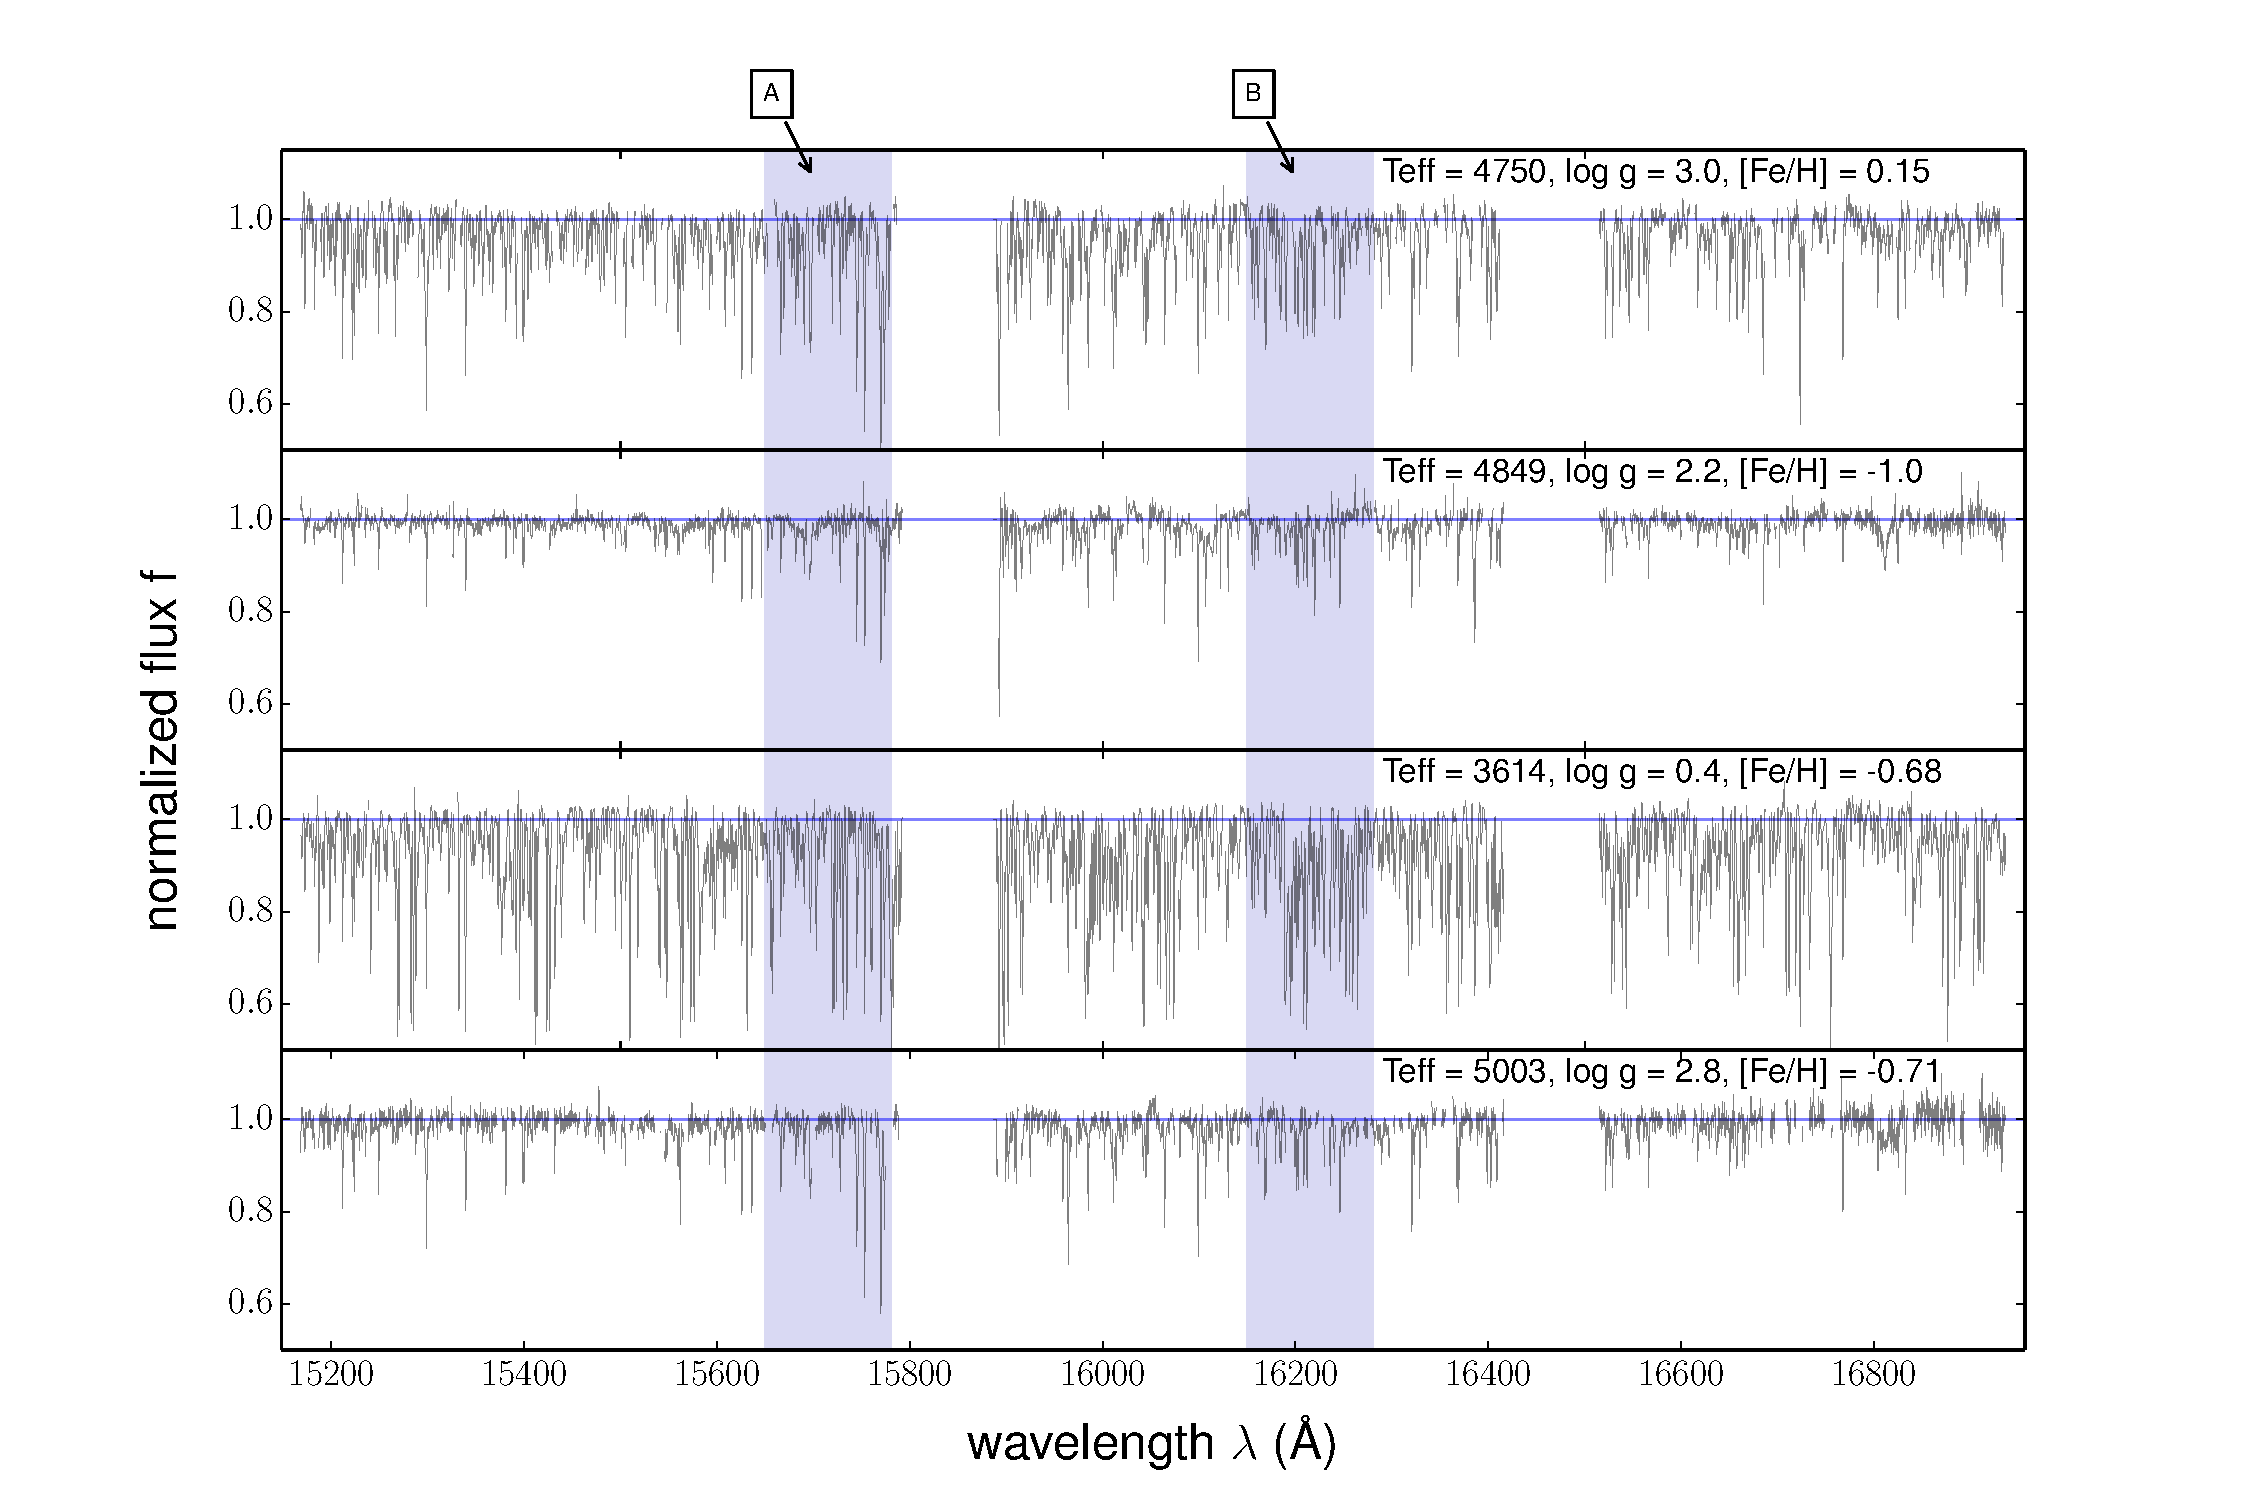
\includegraphics[height=\figureheight]{../documents/plots/four_examples3.pdf}
\end{frame}

\begin{frame}
  \frametitle{train, validate, and test}
  \begin{itemize}
  \item split the data into three disjoint subsets
  \item in the \emph{training step} you set the parameters of your model using the training set
  \item the validation set is used to set hyperparameters or model complexity
  \item in the \emph{test step} you apply the model to the test set---new data---to make predictions or deliver results
  \end{itemize}
\end{frame}

\begin{frame}
  \frametitle{\tc: training set}
  \begin{itemize}
  \item 543 stars (too few) from 19 clusters (too few)
  \item $\teff, \logg, \feh$ labels from \apogee
    \begin{itemize}
    \item calling parameters and abundances ``labels''
    \item slight adjustments to labels to get them onto possible isochrones
    \end{itemize}
  \item \emph{terrible} coverage of the main sequence
    \begin{itemize}
    \item only the Pleiades
    \item home-made Pleiades labels (by Ness)
    \item no $\feh$ spread at high $\logg$.
    \end{itemize}
  \end{itemize}
\end{frame}

\begin{frame}
  \frametitle{\tc: training set}
  ~\hfill\includegraphics<1>[height=\figureheight]{../documents/plots/training_aspcap2.pdf}
         \includegraphics<2>[height=\figureheight]{../documents/plots/training_mkn2.pdf}
\end{frame}

\newcommand{\flux}{f}
\newcommand{\fluxes}{\boldsymbol{\flux}}
\newcommand{\labels}{\boldsymbol{\ell}}
\newcommand{\pars}{\boldsymbol{\theta}}

\begin{frame}
  \frametitle{\tc: model}
  \begin{itemize}
  \item a \emph{generative model} of the \apogee\ spectra
    \begin{itemize}
    \item given label vector $\labels$, predict flux vector $\fluxes$
    \item probabilistic prediction $p(\fluxes\given\labels,\pars)$
    \end{itemize}
  \item use every spectral pixel's uncertainty variance $\sigma^2_{\lambda n}$ responsibly
  \item details:
    \begin{itemize}
    \item spectral expectation is quadratic in the labels
    \item every wavelength $\lambda$ treated independently
    \item an intrinsic Gaussian scatter $s^2_\lambda$ at every wavelength $\lambda$
    \item 80,000 free parameters in $\pars$!
    \end{itemize}
  \end{itemize}
\end{frame}

\begin{frame}
  \frametitle{\tc: model}
  \begin{eqnarray}
    \ln p(\fluxes_n\given\labels_n,\pars) &=& \sum_{\lambda=1}^L \ln p(\flux_{\lambda n}\given\labels_n,\pars_\lambda,s^2_\lambda)
    \nonumber \\
    \ln p(\flux_{\lambda n}\given\labels_n,\pars_\lambda,s^2_\lambda) &=& -\frac{1}{2}\,\frac{[f_{\lambda n} - \transpose{\pars_\lambda}\cdot\labels_n]^2}{\sigma^2_{\lambda n} + s^2_\lambda} + \ln (\sigma^2_{\lambda n} + s^2_\lambda)
    \nonumber \\
    \transpose{\labels} &\equiv& \left\{1, \teff, \logg, \feh, \teff^2, \teff\,\logg, \cdots, \feh^2\right\}
    \nonumber \\
    \transpose{\pars} &\equiv& \left\{\pars_\lambda, s^2_\lambda\right\}_{\lambda=1}^L
    \nonumber
  \end{eqnarray}
  \begin{itemize}
  \item \emph{training step}: optimize parameters $\pars$ at fixed labels
    $\labels$ using training-set data
    \begin{itemize}
    \item linear least squares
    \item every wavelength $\lambda$ treated independently
    \end{itemize}
  \item \emph{test step}: optimize labels $\labels$ at fixed
    parameters $\pars$ using test-set (survey) data
    \begin{itemize}
    \item non-linear optimization
    \end{itemize}
  \end{itemize}
\end{frame}

\begin{frame}
  \frametitle{\tc: model training}
  ~\hfill\includegraphics<1>[height=\figureheight]{./data_model_cyan.png}
\end{frame}

\begin{frame}
  \frametitle{\tc: model training}
  ~\hfill\includegraphics<1>[height=\figureheight]{../documents/plots/R1_continuum5.png}
\end{frame}

\begin{frame}
  \frametitle{\tc: model training cross-validation}
  ~\hfill\includegraphics<1>[height=\figureheight]{../documents/plots/takeout_histc.png}
\end{frame}

\newcommand{\results}{%
\begin{frame}
  \frametitle{\tc: results}
  \begin{itemize}
  \item \tc\ is far faster than physical modeling
    \begin{itemize}
    \item model trains in \emph{seconds} (thousands of least-square fits)
    \item \tc\ labels all 56,000 stars in \apogee\ DR10 in two hours
    \item (pure Python on a laptop)
    \end{itemize}
  \item labels appear sensible
    \begin{itemize}
    \item \tc\ labels lie near sensible isochrones
    \item scatter against \apogee\ labels consistent with \apogee\ precision
    \end{itemize}
  \item successfully puts labels on dwarfs
  \end{itemize}
\end{frame}}

\results

\begin{frame}
  \frametitle{\tc: test time}
  ~\hfill\includegraphics<1>[height=\figureheight]{../documents/plots/4431_v19.png}
         \includegraphics<2>[height=\figureheight]{../documents/plots/4383_v19.png}
         \includegraphics<3>[height=\figureheight]{../documents/plots/4399_v19.png}
         \includegraphics<4>[height=\figureheight]{../documents/plots/4309_v19.png}
         \includegraphics<5>[height=\figureheight]{../documents/plots/4311_v19.png}
         \includegraphics<6>[height=\figureheight]{../documents/plots/4255_v19.png} 
\end{frame}

\begin{frame}
  \frametitle{\tc: comparison with \apogee\ labels}
  ~\hfill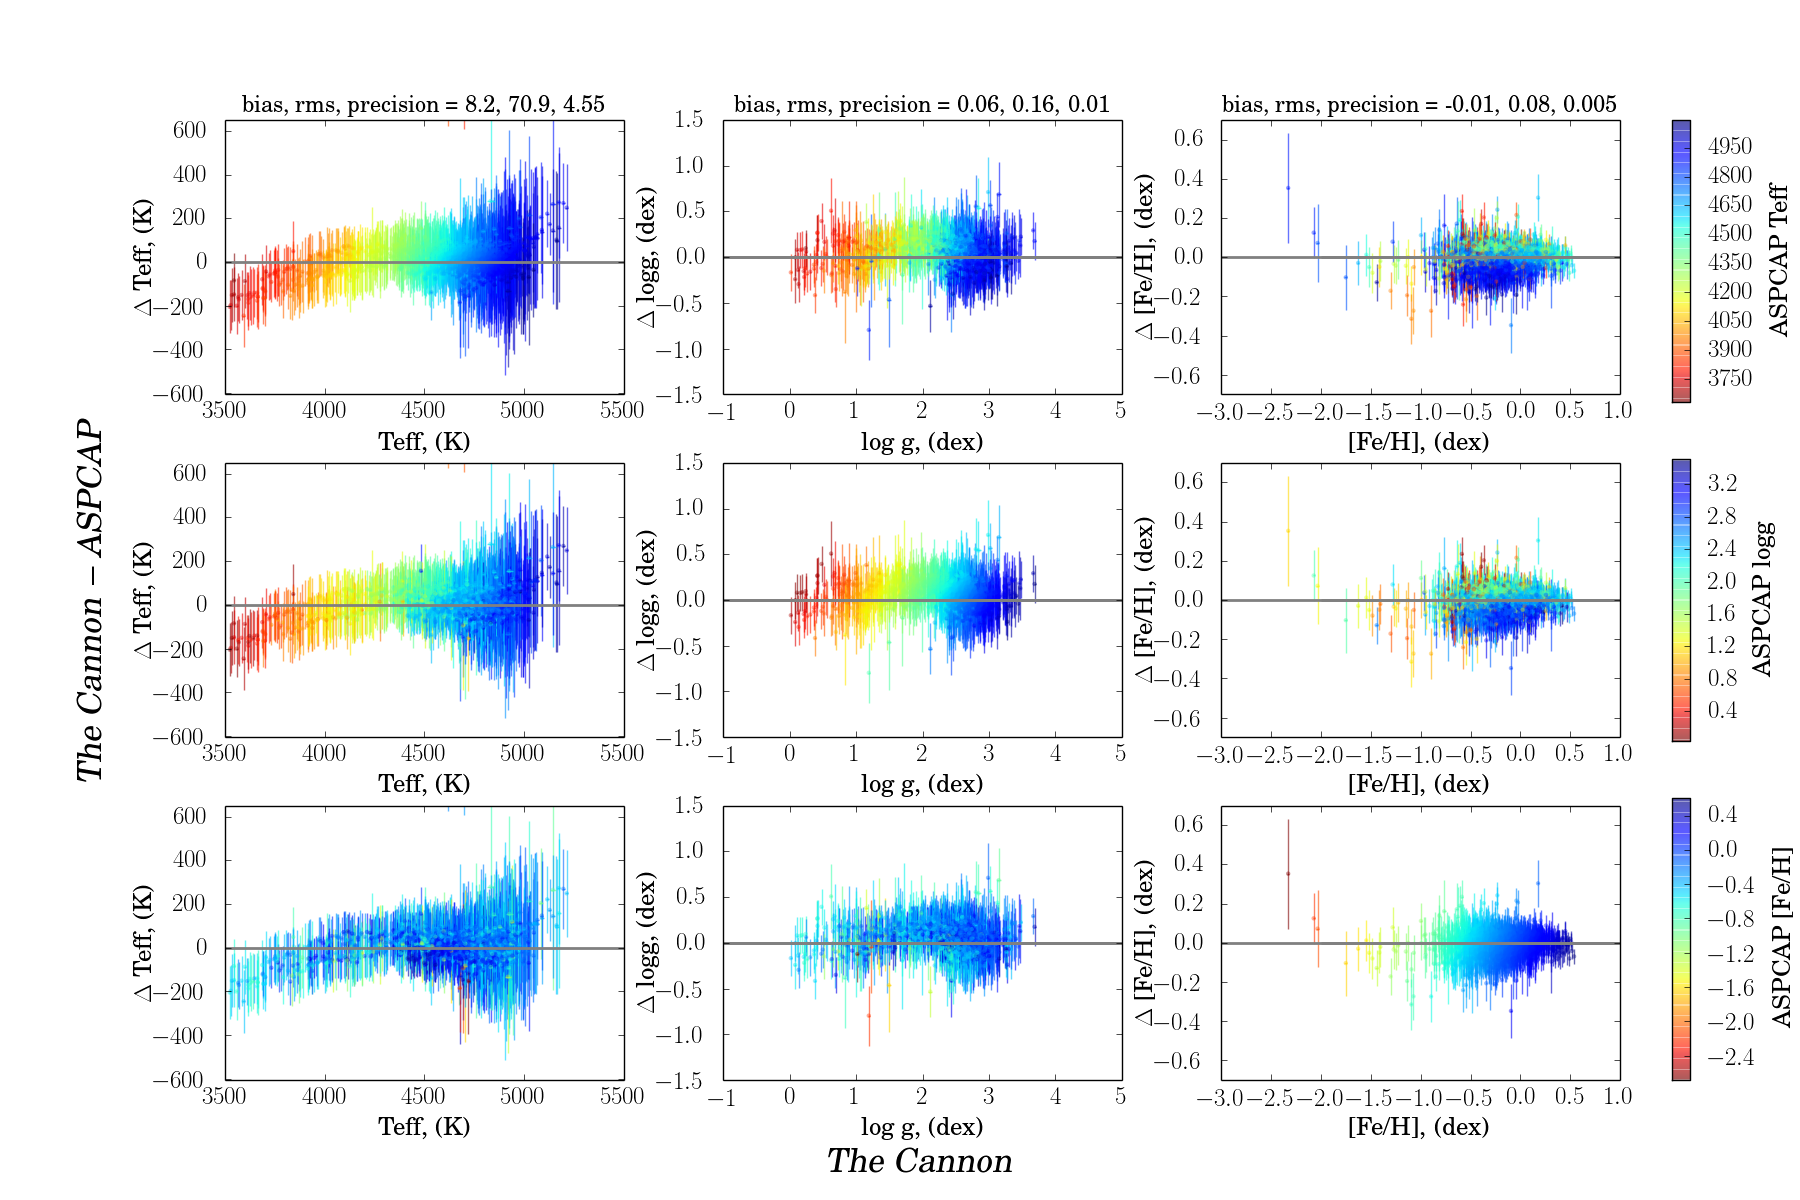
\includegraphics[height=\figureheight]{../documents/plots/cplot2.png} 
\end{frame}

\begin{frame}
  \frametitle{\tc: label veracity}
  ~\hfill\includegraphics<1>[height=\figureheight]{../documents/plots/iso2_2.png}
         \includegraphics<2>[height=\figureheight]{../documents/plots/iso2a_2.png}
\end{frame}

\begin{frame}
  \frametitle{\tc: works at low signal-to-noise}
  ~\hfill\includegraphics<1>[height=\figureheight]{../documents/plots/SNR100to200.png}
         \includegraphics<2>[height=\figureheight]{../documents/plots/SNR20to30.png}
\end{frame}

\begin{frame}
  \frametitle{\tc: label transfer from \apogee\ to \project{LAMOST}}
  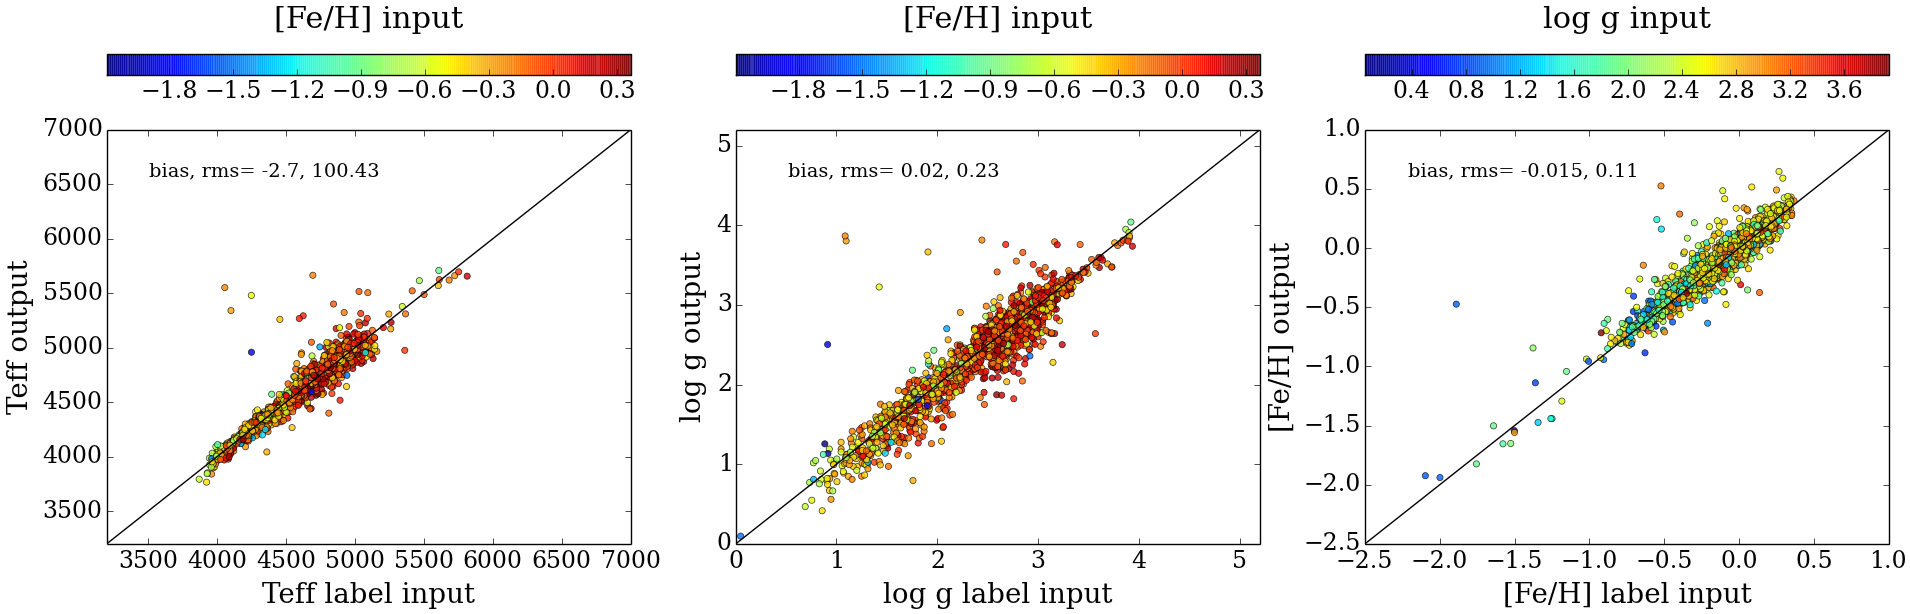
\includegraphics[width=\figurewidth]{LAMOST.png}
\end{frame}

\results

\begin{frame}
  \frametitle{\tc: shortcuts and choices}
  \begin{itemize}
  \item no Bayes; no partial or noisy labels
  \item quadratic order
    \begin{itemize}
    \item replacing polynomial with a Gaussian process (Ho \& Foreman-Mackey)
    \item continuous model complexity; non-parametric
    \end{itemize}
  \item spectral representation
  \item too-small training set
  \item only three labels
    \begin{itemize}
    \item [$\alpha$/Fe], age
    \item splitting the giant branch
    \item how to go to many elements?
    \end{itemize}
  \end{itemize}
\end{frame}

\begin{frame}
  \frametitle{applications for data-driven models}
  \begin{itemize}
  \item \kepler\ and \project{K2} light curves
    \begin{itemize}
    \item the first systematic exoplanet catalog from \project{K2} data
    \item Foreman-Mackey \etal\ (arXiv:1502.04715)
    \end{itemize}
  \item building a consistent all-sky stellar parameter system for \gaia
  \item quasar target selection
    \begin{itemize}
    \item \project{XDQSO} and \project{XDQSOz}
    \item Bovy \etal, 2011 (ApJ 729 141), 2012 (ApJ 749 41)
    \end{itemize}
  \item CMB foregrounds
  \end{itemize}
\end{frame}

\begin{frame}
  \frametitle{data-driven models}
  \begin{itemize}
  \item incredibly powerful tools
    \begin{itemize}
    \item clustering, \emph{label transfer}, prediction, de-noising
    \end{itemize}
  \item make use of things you strongly believe
    \begin{itemize}
    \item especially the noise model
    \end{itemize}
  \item every situation will be \emph{bespoke}
    \begin{itemize}
    \item expect to get dirty
    \end{itemize}
  \end{itemize}
\end{frame}

\end{document}
